\documentclass[10pt,twocolumn,letterpaper]{article}

\usepackage{cvpr}
\usepackage{times}
\usepackage{epsfig}
\usepackage{graphicx}
\usepackage{amsmath}
\usepackage{amssymb}
\usepackage{xcolor}
\usepackage{listings}
\usepackage{hyperref}

% Include other packages here, before hyperref.

% If you comment hyperref and then uncomment it, you should delete
% egpaper.aux before re-running latex.  (Or just hit 'q' on the first latex
% run, let it finish, and you should be clear).
\usepackage[pagebackref,breaklinks,colorlinks,bookmarks=false]{hyperref}

% Support for easy cross-referencing
\usepackage[capitalize]{cleveref}
\crefname{section}{Sec.}{Secs.}
\Crefname{section}{Section}{Sections}
\Crefname{table}{Table}{Tables}
\crefname{table}{Tab.}{Tabs.}
% \cvprfinalcopy % *** Uncomment this line for the final submission

\def\cvprPaperID{****} % *** Enter the CVPR Paper ID here
\def\httilde{\mbox{\tt\raisebox{-.5ex}{\symbol{126}}}}

% Pages are numbered in submission mode, and unnumbered in camera-ready
%\ifcvprfinal\pagestyle{empty}\fi
\setcounter{page}{4321}



\lstdefinestyle{mystyle}{
    language=Python,
    basicstyle=\ttfamily\small,
    commentstyle=\color{green},
    keywordstyle=\color{blue},
    stringstyle=\color{red},
    showstringspaces=false,
    columns=flexible,
}
\lstset{style=mystyle}



\begin{document}

%%%%%%%%% TITLE
\title{Assignment 1: MLP performed on Diabetes Prediction, a Case Study}

\author{Zhengyang li\\
   School of Computer and Mathematical Sciences\\
   Adelaide, South Australia 5005 Australia\\
   \tt\small Zhengyang.li01@adelaide.edu.au}
% For a paper whose authors are all at the same institution,
% omit the following lines up until the closing ``}''.
% Additional authors and addresses can be added with ``\and'',
% just like the second author.
% To save space, use either the email address or home page, not both


\maketitle
%\thispagestyle{empty}

%%%%%%%%% ABSTRACT
\begin{abstract}
   This study elucidates the nuanced interplay between network structure, learning rate, and dropout rate on the performance and generalization of neural network models. Through systematic experimentation, it was observed that a complex network structure, while capable of learning intricate patterns, is prone to overfitting. Dropout, as a regularization technique, mitigates overfitting and enhances model robustness. The choice of learning rate emerged as a trade-off between training efficiency and model performance, necessitating a judicious selection tailored to the specific problem. The findings underscore the significance of prudent network design and hyperparameter tuning in achieving a harmonious balance between model performance and generalization, thereby informing better practices for constructing and evaluating neural network models for robust real-world deployments. Note that all the file can be found on the : \href{https://github.com/David-Lzy/Deep_Learning_Fundamentals}{Github}
\end{abstract}

%%%%%%%%% BODY TEXT
5\section{Introduction}

The realm of Artificial Intelligence (AI) has undergone remarkable advancements over the past few decades, with Neural Networks (NNs) spearheading this technological evolution. Tracing back to the 1940s, the inception of neural networks was fueled by the human brain's intricate neuron structure. Early models aspired to emulate the brain's capacity to learn from and interpret data. As computational power and data availability burgeoned over time, neural networks morphed into sophisticated architectures capable of tackling complex problems across a myriad of domains.

A pivotal milestone in the annals of neural networks is the advent of the Perceptron algorithm by Frank Rosenblatt in 1957~\cite{Crowell1965, Rhee1976}. Often hailed as the rudimentary form of a neural network, the Perceptron is a binary linear classifier that paved the way for the emergence of Multi-layer Perceptrons (MLPs) and, subsequently, deep learning~\cite{Boubiche1969}. The elegance of the algorithm resides in its simplicity and the ability to discern linearly separable patterns through an iterative process of weight adjustments predicated on the input data~\cite{Boubiche1969, McMillen1968}.

The quintessence of a Perceptron hinges on the notion of a linear decision boundary. It operates by attributing weights to input features, aggregating the weighted inputs, applying a step function, and rendering a binary decision. The learning trajectory of the Perceptron entails adjusting the weights predicated on the prediction errors, steering the model towards a state wherein all the training exemplars are accurately classified, given the data is linearly separable.

Over the epochs, the Perceptron algorithm has acted as a catalyst propelling towards more sophisticated neural network architectures and learning algorithms. Its legacy continues to shed light on the design and comprehension of contemporary neural networks and deep learning models. The transition from rudimentary linear classifiers like the Perceptron to today's elaborate deep learning architectures epitomizes the relentless endeavor to mimic human cognitive faculties and propel the field of artificial intelligence forward~\cite{Du2022}.

The battle against diabetes, a chronic disease characterized by elevated blood sugar levels, has been a long-standing endeavor in the medical community\cite{Kang2021, Elghamrawy2020}. The early 20th century saw the discovery of insulin, a significant milestone that transformed diabetes from a fatal disease to a manageable condition. However, with the prevalence of diabetes surging globally, the need for more sophisticated methods of prediction and management became apparent. The evolution of computational power and data science methodologies in recent decades has fostered a conducive environment for the application of machine learning and artificial intelligence (AI) in diabetes research\cite{Bukhari2021}.

One pioneering stride in this domain was the application of machine learning algorithms to predict the onset of diabetes based on various risk factors. The dataset provided in the assignment, encapsulating features like glucose levels, blood pressure, and body mass index, serves as a testament to the early efforts in employing data-driven approaches to understand and predict diabetes. Algorithms like logistic regression, support vector machines, and neural networks were employed to unearth the underlying patterns in the data, aiding in early diagnosis and personalized treatment plans.

The advent of the Perceptron algorithm, as discussed in the preceding sections, marked a significant point in the journey towards leveraging neural networks for medical diagnoses, including diabetes. The Perceptron, with its ability to delineate linear decision boundaries, provided a simplistic yet effective approach towards understanding the relationships between various risk factors and the onset of diabetes. Over time, with the emergence of deep learning, more complex and nuanced models were developed, capable of handling multi-dimensional data and providing more accurate predictions.

The continuum of research in diabetes prediction using AI has not only enhanced the accuracy and timeliness of diagnoses but also shed light on the intricate interplay of various risk factors contributing to the disease. The present assignment delves into the implementation of the Perceptron algorithm to predict diabetes, standing at the intersection of historical advancements in both neural networks and diabetes research. The endeavor encapsulates the ongoing pursuit of better understanding, predicting, and managing diabetes, showcasing the potential of AI in tackling real-world healthcare challenges.

This paper is structured as follows: Section 2 delineates the fundamental principles underlying the construction of neural networks, with subsections 2.1 and 2.2 expounding on linear combination and activation functions respectively. Section 3 chronicles the experimental setup, where subsection 3.1 discusses the data analysis and cleansing process, followed by subsection 3.2 which delineates the implementation of the model. Section 4 presents the results of the study, with subsections 4.1, 4.2, and 4.3 delving into the influences of network complexity, learning rate, and dropout rate on model performance and generalization, respectively. Lastly, Section 5 encapsulates the key findings and conclusions derived from the experiments, offering a synthesis of the insights garnered pertaining to the design and evaluation of neural network models.

\section{Method}

The Single-layer Perceptron (SLP) is a rudimentary form of a neural network and serves as a linear classifier. At its core, the SLP operates based on two primary components: linear combination and activation function, which are crucial in understanding the architecture's ability to perform binary classification.

\subsection{Linear Combination}
The first step in the perceptron algorithm is to perform a linear combination of the input features and weights, possibly with a bias term. The formula for the linear combination is given by:
\[
   z = \sum_{i=1}^{n} w_i x_i + b
\]
where:
\begin{itemize}
   \item \( n \) is the number of input features,
   \item \( x_i \) are the input features,
   \item \( w_i \) are the weights associated with the input features,
   \item \( b \) is the bias term.
\end{itemize}
This mechanism bears resemblance to traditional linear regression, where a similar linear combination of input features is used to predict a continuous target variable. Both models aim to find the optimal set of weights that minimize the error between the predicted values and the actual values. However, while linear regression stops at this linear combination to produce its output, the perceptron takes this output further through an activation function, transitioning from a continuous domain to binary classification.

\subsection{Activation Function}
The result \( z \) from the linear combination is passed through an activation function, typically the Sigmoid function, to produce the output.

Below, we delve into three common activation functions: Sigmoid, Hyperbolic Tangent (Tanh), and Rectified Linear Unit (ReLU), outlining their distinct characteristics and comparing their effects on the output of a single-layer perceptron using the fruit classification example. Note, the \( z \) in the following formula is result from the linear combination.

\textbf{Sigmoid:}
The sigmoid activation function, also known as the logistic function, maps its input into a range between 0 and 1, which can be used to estimate probabilities. The formula for the sigmoid function is given by:
\[
   \sigma(z) = \frac{1}{{1 + e^{-z}}}
\]

\textbf{Hyperbolic Tangent (Tanh):}
The hyperbolic tangent (tanh) activation function scales its input to a range between -1 and 1. It's essentially a scaled version of the sigmoid activation function. The formula for the tanh function is given by:
\[
   \tanh(z) = \frac{{e^{z} - e^{-z}}}{{e^{z} + e^{-z}}}
\]

\textbf{Rectified Linear Unit (ReLU):}
The Rectified Linear Unit (ReLU) activation function outputs the input directly if it is positive; otherwise, it will output zero. It has become the default activation function for many types of neural networks because a model that uses ReLU can often converge faster. The formula for the ReLU function is given by:
\[
   \text{ReLU}(z) = \max(0, z)
\]

The performance and learning capability of neural networks hinge significantly on the choice of activation functions. These functions introduce non-linearity to the model, which is pivotal for learning complex patterns and making sophisticated decisions beyond mere linear separations. In order to make the results of the activation function clear, a demo is performed to scrutinize the impact of diverse activation functions on the output of a single-layer perceptron. In the provided table, four distinct activation functions—Linear (None), Sigmoid, Hyperbolic Tangent (Tanh), and Rectified Linear Unit (ReLU)—are evaluated across a range of input values \( z \) from -1.0 to 0.8. The following discussion elaborates on the behaviors and implications of these activation functions, as revealed by the tabulated outputs.

\begin{table}[h]
   \centering
   \begin{tabular}{|c|c|c|c|c|}
      \hline
      Input \( z \) & None  & Sigmoid & Tanh  & ReLU \\
      \hline
      -1.00         & -1.00 & 0.27    & -0.76 & 0.00 \\
      -0.70         & -0.70 & 0.33    & -0.60 & 0.00 \\
      -0.40         & -0.40 & 0.40    & -0.38 & 0.00 \\
      -0.10         & -0.10 & 0.48    & -0.10 & 0.00 \\
      0.20          & 0.20  & 0.55    & 0.20  & 0.20 \\
      0.50          & 0.50  & 0.62    & 0.46  & 0.50 \\
      0.80          & 0.80  & 0.69    & 0.66  & 0.80 \\
      \hline
   \end{tabular}
   \caption{Comparison of different activation functions.}
   \label{tab:activation_functions}
\end{table}

The Linear function, serving as a baseline, directly outputs the input value $f(z) = ( z )$ . While simple, it lacks the non-linearity essential for capturing complex data patterns. Its unbounded output range could potentially lead to escalating values during training, hindering the convergence to optimal weights. On the other hand, the Sigmoid function maps the input into a bounded range between 0 and 1, making it a suitable choice for binary classification tasks. However, it's susceptible to the vanishing gradient problem, wherein the gradients become negligibly small for extreme input values, impeding the learning process. Moreover, the Sigmoid function is not zero-centered, which could potentially result in a zig-zagging trajectory during optimization, prolonging the convergence.

Contrastingly, the Tanh function ameliorates the zero-centered issue by mapping the input values between -1 and 1. Although it still suffers from the vanishing gradient problem, the issue is less pronounced compared to the sigmoid function. The zero-centered nature of the Tanh function usually expedites convergence, rendering it a preferable choice over the sigmoid for certain applications. The Rectified Linear Unit (ReLU) function, known for its simplicity, outputs the input directly if positive; otherwise, it outputs zero. This piecewise linear function has gained popularity due to its ability to mitigate the vanishing gradient problem significantly. However, it's not devoid of challenges; a notable one being the dying ReLU problem where neurons get stuck during training, always outputting zero. This issue is alleviated in ReLU variants such as Leaky ReLU.

\subsection{Multi-layer Perceptrons}

The conceptualization and application of neural networks are deeply entrenched in the architectural differences between Single-layer Perceptrons (SLP) and Multi-layer Perceptrons (MLP). These architectures delineate the boundaries of linear and non-linear decision domains, significantly impacting the complexity of tasks that can be undertaken. Multi-layer Perceptrons (MLP) are more intricate, encompassing multiple layers of neurons, each with its own set of weights and activation function. An MLP consists of at least one hidden layer in addition to the input and output layers, thereby introducing multiple levels of computations and non-linearities. The expression for an MLP with one hidden layer is delineated as:

\[
   h_j = \sigma \left( \sum_{i=1}^{n} w_{ji} x_i + b_j \right) \quad \text{for } j = 1, \ldots, m
\]

\[
   \hat{y}_k = \sigma \left( \sum_{j=1}^{m} v_{kj} h_j + c_k \right) \quad \text{for } k = 1, \ldots, p.
\]

Here, $h_j$ are the hidden layer neurons, $m$ is the number of neurons in the hidden layer, $v_{kj}$ are the weights connecting the hidden layer to the output layer, $p$ is the number of output neurons, and $c_k$ is the bias term for the output layer. The inclusion of hidden layers imbues MLPs with the capability to learn non-linear decision boundaries, thus enabling them to tackle more complex, non-linearly separable tasks.

\section{Experiencenment}

\subsection{Data analysis and clean}

\begin{figure}[htbp]
   \centering
   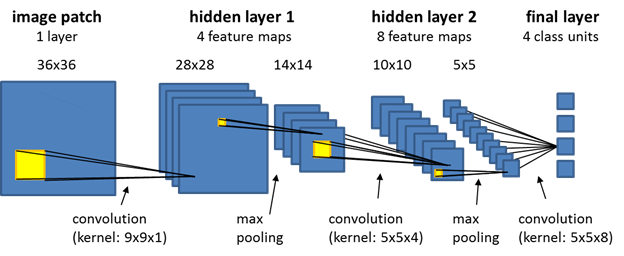
\includegraphics[width=0.5\textwidth]{Fig/1.png}
   \caption{Box plot of standardized features} \label{fig1}
\end{figure}

\subsection{Model Implementation}

The initial step in our data analysis involved loading the dataset from a CSV file and examining its structure to understand the available features and the nature of the data. The dataset comprises several features, namely Pregnancies, Glucose, BloodPressure, SkinThickness, Insulin, BMI (Body Mass Index), DiabetesPedigreeFunction, and Age, along with the target variable Outcome, which indicates the presence (1) or absence (0) of diabetes. An initial inspection of the data revealed that certain features had a value of zero, which is biologically implausible. This anomaly was particularly observed in the features Glucose, BloodPressure, SkinThickness, Insulin, and BMI, suggesting that these zero values represent missing data.

To address the issue of missing values, a decision was made to replace the zeros in the aforementioned features with NaN (Not a Number), which allows for a more accurate computation of statistics such as the median. Following this, the median value of each of these features was computed and used to replace the NaN entries. This strategy for handling missing values is a common practice as it minimizes the distortion of the data distribution, thereby preserving the original structure of the data to a significant extent.

With the missing values appropriately handled, the next step was to standardize the dataset. Standardization is a crucial preprocessing step, especially in the context of neural network models, as it scales the data to have a mean of 0 and a standard deviation of 1. This scaling was applied to all features except the Outcome variable, which is the target variable for our predictive model. The standardization process aids in ensuring that the Perceptron algorithm's performance is not adversely affected by the original scale of the features.

Post-standardization, a visual inspection was carried out to identify any potential outliers in the data. A box plot of the standardized features was generated, providing a clear visualization of the data's distribution and any existing outliers. Outliers can significantly affect the performance of machine learning algorithms, and identifying them is a critical step in the data analysis process.

The data analysis process outlined above is fundamental in preparing the data for the subsequent implementation of the Perceptron algorithm. Through meticulous handling of missing values, standardization of the dataset, and visual identification of outliers, we ensured that the data is in a suitable format for training the predictive model. This preprocessing pipeline is instrumental in ensuring the reliability and accuracy of the predictions generated by the Perceptron algorithm in the task of diabetes prediction.

The implementation of the perceptron model, training, and evaluation are critical steps towards understanding and analyzing the behavior and performance of neural networks in solving complex tasks. This section delineates the process of implementing a single-layer perceptron, structuring the training loop, and evaluating the model using a well-structured codebase. The provided code is written in PyTorch, a powerful and flexible open-source machine learning library, which facilitates the implementation and evaluation of neural network models.

The core of the implementation is the definition of the perceptron model. This is encapsulated within a class named Perceptron, which inherits from nn.Module, the base class for all neural network modules in PyTorch. The perceptron model is characterized by a single linear layer defined using nn.Linear, which computes the weighted sum of its input (a linear combination of the input features and model weights), adds a bias, and passes the result through a sigmoid activation function. The sigmoid activation function ensures that the output of the model is bounded between 0 and 1, making it suitable for binary classification tasks. The forward method of the Perceptron class defines the forward pass of the model, which is the computation performed to generate an output from the input data.


\begin{lstlisting}
   import torch
   import torch.nn as nn
   
   class Perceptron(nn.Module):
       def __init__(self, input_dim):
           super(Perceptron, self).__init__()
           self.fc1 = nn.Linear(input_dim, 1)
       
       def forward(self, x):
           out = torch.sigmoid(self.fc1(x))
           return out

   \end{lstlisting}

To instantiate the perceptron model, a separate class named Trainer encapsulates the training infrastructure, including the preparation of data, definition of loss function, and optimizer. The training data is loaded using a DataLoader, which facilitates batch processing, shuffling of data, and parallel processing. The BCELoss (Binary Cross Entropy Loss) is chosen as the loss function as it is well-suited for binary classification tasks. The Adam optimizer is employed to adjust the model parameters to minimize the loss function during training.

\begin{lstlisting}
   class Trainer:
   def __init__(...):
       ...
       self.criterion = nn.BCELoss()
       self.optimizer = optim.Adam(
         self.model.parameters(), 
         lr=learning_rate
         )
   ...
   \end{lstlisting}

The train method of the Trainer class defines a single epoch of training, wherein the model parameters are adjusted to minimize the loss over the training data. The run method encapsulates the main training loop, iterating over a specified number of epochs, and evaluating the model at specified intervals.
\begin{lstlisting}
   ...
   def train(self):
      ...
      for inputs, targets in self.train_loader:
         ...
         loss.backward()
         self.optimizer.step()
      ...

   def run(self, num_epochs, interval):
      ...
      for epoch in range(num_epochs):
         ...
         if (epoch + 1) % interval == 0:
            self.evaluate(...)
   ...
   \end{lstlisting}
Similarly, the evaluate method of the Trainer class evaluates the model on the validation data, computing the loss and accuracy. The accuracy is computed by comparing the model's predictions with the actual labels, and the average loss and accuracy are returned as the evaluation metrics.

To investigate how the the layer and the corresponding neurons impact on the model's performance, a Multi-layer Perceptron (MLP) using the PyTorch library model was trained with series number of layers and neurons. The number of layers was varied from 1 to 6, and the number of neurons was varied between 1 and 64. The loss and accuracy were recorded for each combination of layers and neurons.
\begin{lstlisting}
   class MLP_fix(nn.Module):
   def __init__(
      self, 
      input_dim, 
      hidden_dim, 
      num_layers
      ):
       ...
       for i in range(num_layers - 1):
           self.layers.append(
            nn.Linear(hidden_dim, hidden_dim)
            )
       ...
       self.fc_last = nn.Linear(hidden_dim, 1)
   ...
    def forward(self, x):
        ...
        for layer in self.layers:
            x = torch.relu(layer(x))
        ...
        out = torch.sigmoid(self.fc_last(x))
        return out
    ...
   \end{lstlisting}
Note, all the experiences were performed on my serevr, which equipped with an Intel Xeon E5-2696 v3 CPU * 2, an NVIDIA RTX 3090 GPU, and 256GB of RAM. The system operates on Ubuntu 22.04 LTS, and the code was written in Python 3.10, PyTorch 2.0 and CUDA 11.8.

\section{Results}

The results presented elucidate the impact of varying network structures on the performance of the implemented Multi-layer Perceptron (MLP) model across multiple metrics including training loss, training accuracy, testing accuracy, and execution time.

\begin{table*}[h]
   \centering
   \begin{tabular}{|c|c|c|c|c|c|}
      \hline
      Net Structure & Training Loss & Training Accuracy & Testing Accuracy & Duration (sec) \\
      \hline
      (2,)          & 44.52\%       & 78.83\%           & 69.48\%          & 4.09           \\
      (4,)          & 41.49\%       & 79.97\%           & 75.97\%          & 3.93           \\
      (8,)          & 41.69\%       & 80.46\%           & 71.43\%          & 3.96           \\
      (16,)         & 39.98\%       & 80.94\%           & 76.62\%          & 3.96           \\
      (32,)         & 36.47\%       & 83.06\%           & 74.68\%          & 3.97           \\
      (64,)         & 34.02\%       & 84.53\%           & 74.03\%          & 4.16           \\
      \hline
   \end{tabular}
   \caption{Results of different network structures.}
   \label{tab:net_struct_results}
\end{table*}

\subsection{Influence of the number of layers and neurons}

\begin{table*}[h]
   \centering
   \begin{tabular}{|c|c|c|c|c|}
      \hline
      Net Structure                 & Training Loss & Training Accuracy & Testing Accuracy & Duration (sec) \\
      \hline
      (16, 16)                      & 32.91\%       & 84.69\%           & 72.73\%          & 4.88           \\
      (16, 32, 16)                  & 18.42\%       & 93.32\%           & 74.03\%          & 5.53           \\
      (16, 32, 32, 16)              & 6.29\%        & 98.37\%           & 70.13\%          & 6.75           \\
      (16, 32, 64, 32, 16)          & 0.62\%        & 100.00\%          & 66.88\%          & 7.49           \\
      (16, 32, 64, 64, 32, 16)      & 0.13\%        & 100.00\%          & 67.53\%          & 9.04           \\
      (16, 32, 64, 128, 64, 32, 16) & 0.03\%        & 100.00\%          & 68.83\%          & 10.52          \\
      \hline
   \end{tabular}
   \caption{Results of different network structures.}
   \label{tab:net_struct_results}
\end{table*}

The network structure evidently plays a pivotal role in the model's performance. As the complexity of the network structure increases (from 2 to 64 neurons), there is a discernible decline in training loss (from 44.52\% to 34.02\%) and a concomitant improvement in training accuracy (from 78.83\% to 84.53\%). This trend underscores the enhanced capacity of more complex networks to capture underlying patterns in the training data, hence resulting in better training performance. Additionally, the set of experiments introduces additional hidden layers into the MLPs, thereby increasing the network's depth. As observed, a deeper network structure tends to achieve lower training loss and higher training accuracy, culminating in a perfect training accuracy of 100\% for the three deepest networks. This underscores the capacity of deeper networks to better fit the training data. However, the improvement in training performance comes at the cost of longer training durations. The execution time progressively increases with the complexity of the network, demonstrating the computational overhead associated with deeper and more complex networks.


The training loss exhibits a precipitous decline as the network structure becomes more complex, particularly transitioning from a single hidden layer to multiple hidden layers. The training loss drops from 32.91\% to a negligible 0.03\%, underlining the model's increasing aptitude in minimizing the error between the predicted and actual outcomes in the training dataset. This disparity is indicative of overfitting, a common ailment in deep learning where the model learns to memorize the training data at the expense of generalization to unseen data.

The results reinforce the notion of a trade-off between network complexity and model generalization. While complex networks exhibit superior training performance, they are prone to overfitting, which deteriorates their testing accuracy. The result suggest that there exists an optimal point in the network complexity spectrum where the model achieves a respectable balance between fitting the training data and generalizing to unseen data, as evidenced by the network structure (16, 32, 16).

\subsection{Influence of the learning rate}

\begin{figure*}[htbp]
   \centering
   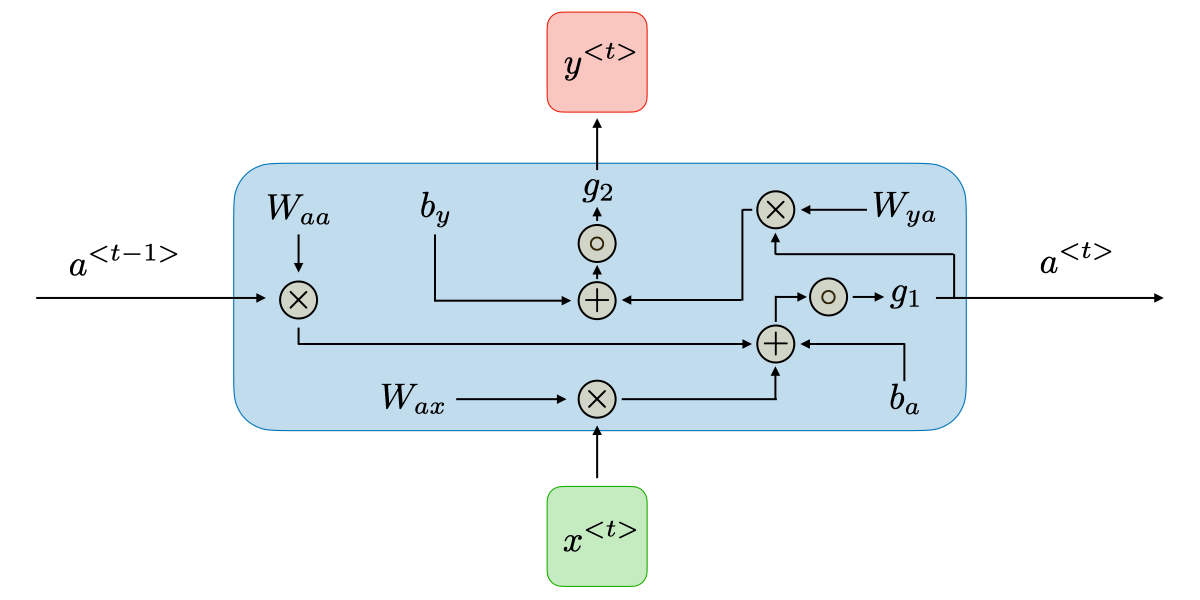
\includegraphics[width=0.99\textwidth]{Fig/2.png}
   \caption{Plot of Convergence Speed, Training and Testing Accuracy with series learning rate.} \label{fig2}
\end{figure*}

Upon reviewing the graphical representation of the effect of different learning rates on the training loss, training accuracy, and testing accuracy, several key insights emerge that elucidate the nuanced role that learning rate plays in the convergence and performance of the neural network model.

As we can see in Fig.2, the plots distinctly reveal that a smaller learning rate extends the time required for the model to converge. This is in alignment with the inherent working mechanism of gradient descent optimization, where a smaller learning rate implies smaller steps toward the minimum of the loss function. The slower convergence associated with smaller learning rates can be perceived as a meticulous examination of the loss landscape, which although time-consuming, often leads to a more precise convergence to the global or local minima. Conversely, a higher learning rate expedites the convergence but at the risk of overshooting the minima or oscillating around it. This rapid convergence, though computationally efficient, may settle at suboptimal points in the loss landscape, thus potentially compromising the model's performance.

The insights derived from the plots underscore the importance of an appropriately chosen learning rate in training neural networks. An excessively high learning rate might lead to rapid but suboptimal convergence, while an exceedingly low learning rate, despite ensuring meticulous convergence, could be computationally prohibitive especially in real-world scenarios with time constraints.

\subsection{Influence of the dropout rate}

\begin{figure*}[htbp]
   \centering
   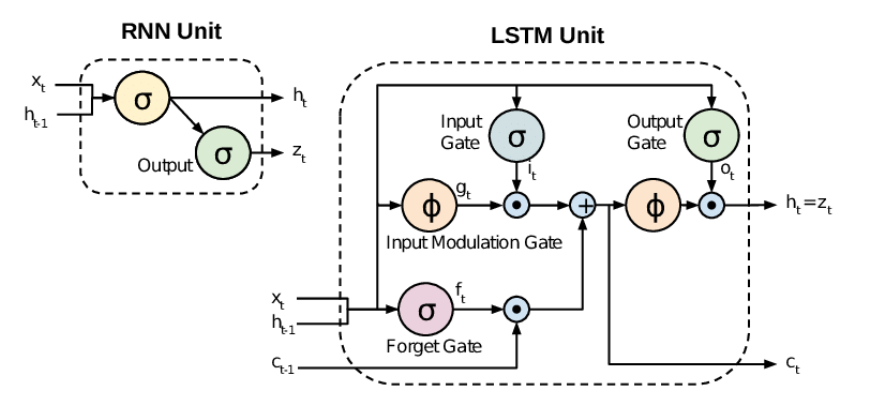
\includegraphics[width=0.99\textwidth]{Fig/3.png}
   \caption{Plot of Convergence Speed, Training and Testing Accuracy with series drop rate.} \label{fig3}
\end{figure*}

Here in Fig.3, the influence of varying dropout rates on the training loss, training accuracy, and testing accuracy, were presented here. The plots vividly delineate that a lower dropout rate facilitates a swifter convergence during the training phase. This phenomenon is underpinned by the fact that a lower dropout rate retains a larger portion of neurons active during training, thereby accelerating the learning process. However, this expedited convergence comes at the peril of overfitting, especially when the model is exposed to a complex or noisy data landscape. The overfitting peril emanates from the model's propensity to memorize the training data rather than generalizing from it, a scenario exacerbated by a lower dropout rate.

The plots further expound that a higher dropout rate engenders a more robust model that generalizes well to unseen data as manifested in the testing accuracy plot. The essence of dropout as a regularization technique is to prevent the co-adaptation of features by randomly dropping out neurons, thereby promoting the model's ability to generalize. The increment in testing accuracy with higher dropout rates evinces the efficacy of dropout in mitigating overfitting, albeit at the expense of a slower convergence and potentially a slightly compromised training accuracy. The gradual ascension in testing accuracy with higher dropout rates accentuates the trade-off between model complexity and generalization. While a lower dropout rate might yield higher training accuracy due to lower model regularization, it doesn’t transmute into better testing accuracy, underscoring the overfitting dilemma.


\section{Summary and Conclusion}

In conclusion, the journey through varying network structures, learning rates, and dropout rates sheds light on the nuanced interplay of these factors in model training and performance. The exploration of different network structures underpins the balance between complexity and generalization. As the network deepens or widens, the capacity to learn intricate patterns increases, yet at the peril of overfitting to the training data. This scenario is especially palpable in networks with a larger number of neurons, where the training loss dwindles, but the testing accuracy doesn't see a commensurate improvement. The discrepancy in performance between the training and testing datasets is indicative of overfitting, a phenomenon that is mitigated to a certain extent with an increasing dropout rate. Dropout, as a regularization technique, injects a level of robustness into the model by promoting the learning of more generalized features, thus enhancing the model's performance on unseen data.

The analysis also underscores the cardinal role of the learning rate in the training dynamics. A smaller learning rate, although ensuring a more meticulous convergence, demands a longer training duration. On the flip side, a higher learning rate expedites the training process but at the cost of possibly overshooting the global minimum of the loss function or oscillating around it. The choice of learning rate is hence a trade-off between training efficiency and model performance, necessitating a judicious selection tailored to the specific problem and data at hand. The graphical representation vividly illustrates this trade-off, offering a visual narrative on the importance of an apt learning rate selection.

Furthermore, the comparison between different dropout rates unveils a compelling narrative on model regularization. A higher dropout rate, although slowing down the training, imparts a level of resistance to overfitting, ensuring that the model learns a more generalized representation of the data. Conversely, a lower dropout rate speeds up convergence but is more susceptible to overfitting, especially in complex networks. The graphical elucidation of the dropout rate effect accentuates the significance of dropout as a regularization tactic, fostering not only a robust learning from the training data but also an enhanced generalization to unseen data. This, in turn, bolsters the model's predictive accuracy and robustness, paving the way for more reliable deployments in real-world scenarios. Through a meticulous analysis and a visual narrative, the results delineate the essence of prudent network design and hyperparameter tuning in sculpting neural network models that are adept at both learning and generalizing across varying data landscapes.




   {\small
      \bibliographystyle{ieee_fullname}
      \bibliography{egbib}
   }


\end{document}
